\section*{Problem A}\label{sec:introduction}


\textit{Select the checkerboard pattern for the data, which is known as the XOR dataset. The data is sampled from a 2D probability density distribution represented by $(x_1, x_2)$. The regions $x_1, x_2 > 0$ and $x_1, x_2 < 0$ have a target value $y = +1$ and are shown as blue data points, while the regions $x_1 > 0, x_2 < 0$ and $x_1 < 0, x_2 > 0$ have a target value of $y = -1$ and are shown as orange data points.}

\textit{First, select a linear model with no hidden layers. For the features, select the two independent variables x1 and x2. Can you fit the data with this linear model? Why or why not? What happens if you add the feature $x_1x_2$?}


We can see that data will never be fitted with the linear model (Figure \ref{fig:x1_x2_feat}) as both the training loss and test loss are about the same. This implies that the model has a high bias always underfitting, meaning it has a high bias. More fundamentally, the data requires $y=+1$ when $x_1\cdot x_2>0$ and $y=-1$ for $x_1\cdot x_2<0$. This can never be acheived with only a linear model of the independent variables $x_1$ and $x_2$ as features. Therefore, a combination of the variables as a new additional feature is necessary e.g. $x_1x_2$. This is shown in Figure \ref{fig:x1_x2_x1x2_feat}. We see that after 1,025 epochs, the neural network fits the training data "perfectly" with a test loss of 0.002. 
\begin{figure}[htbp]
    \centering
    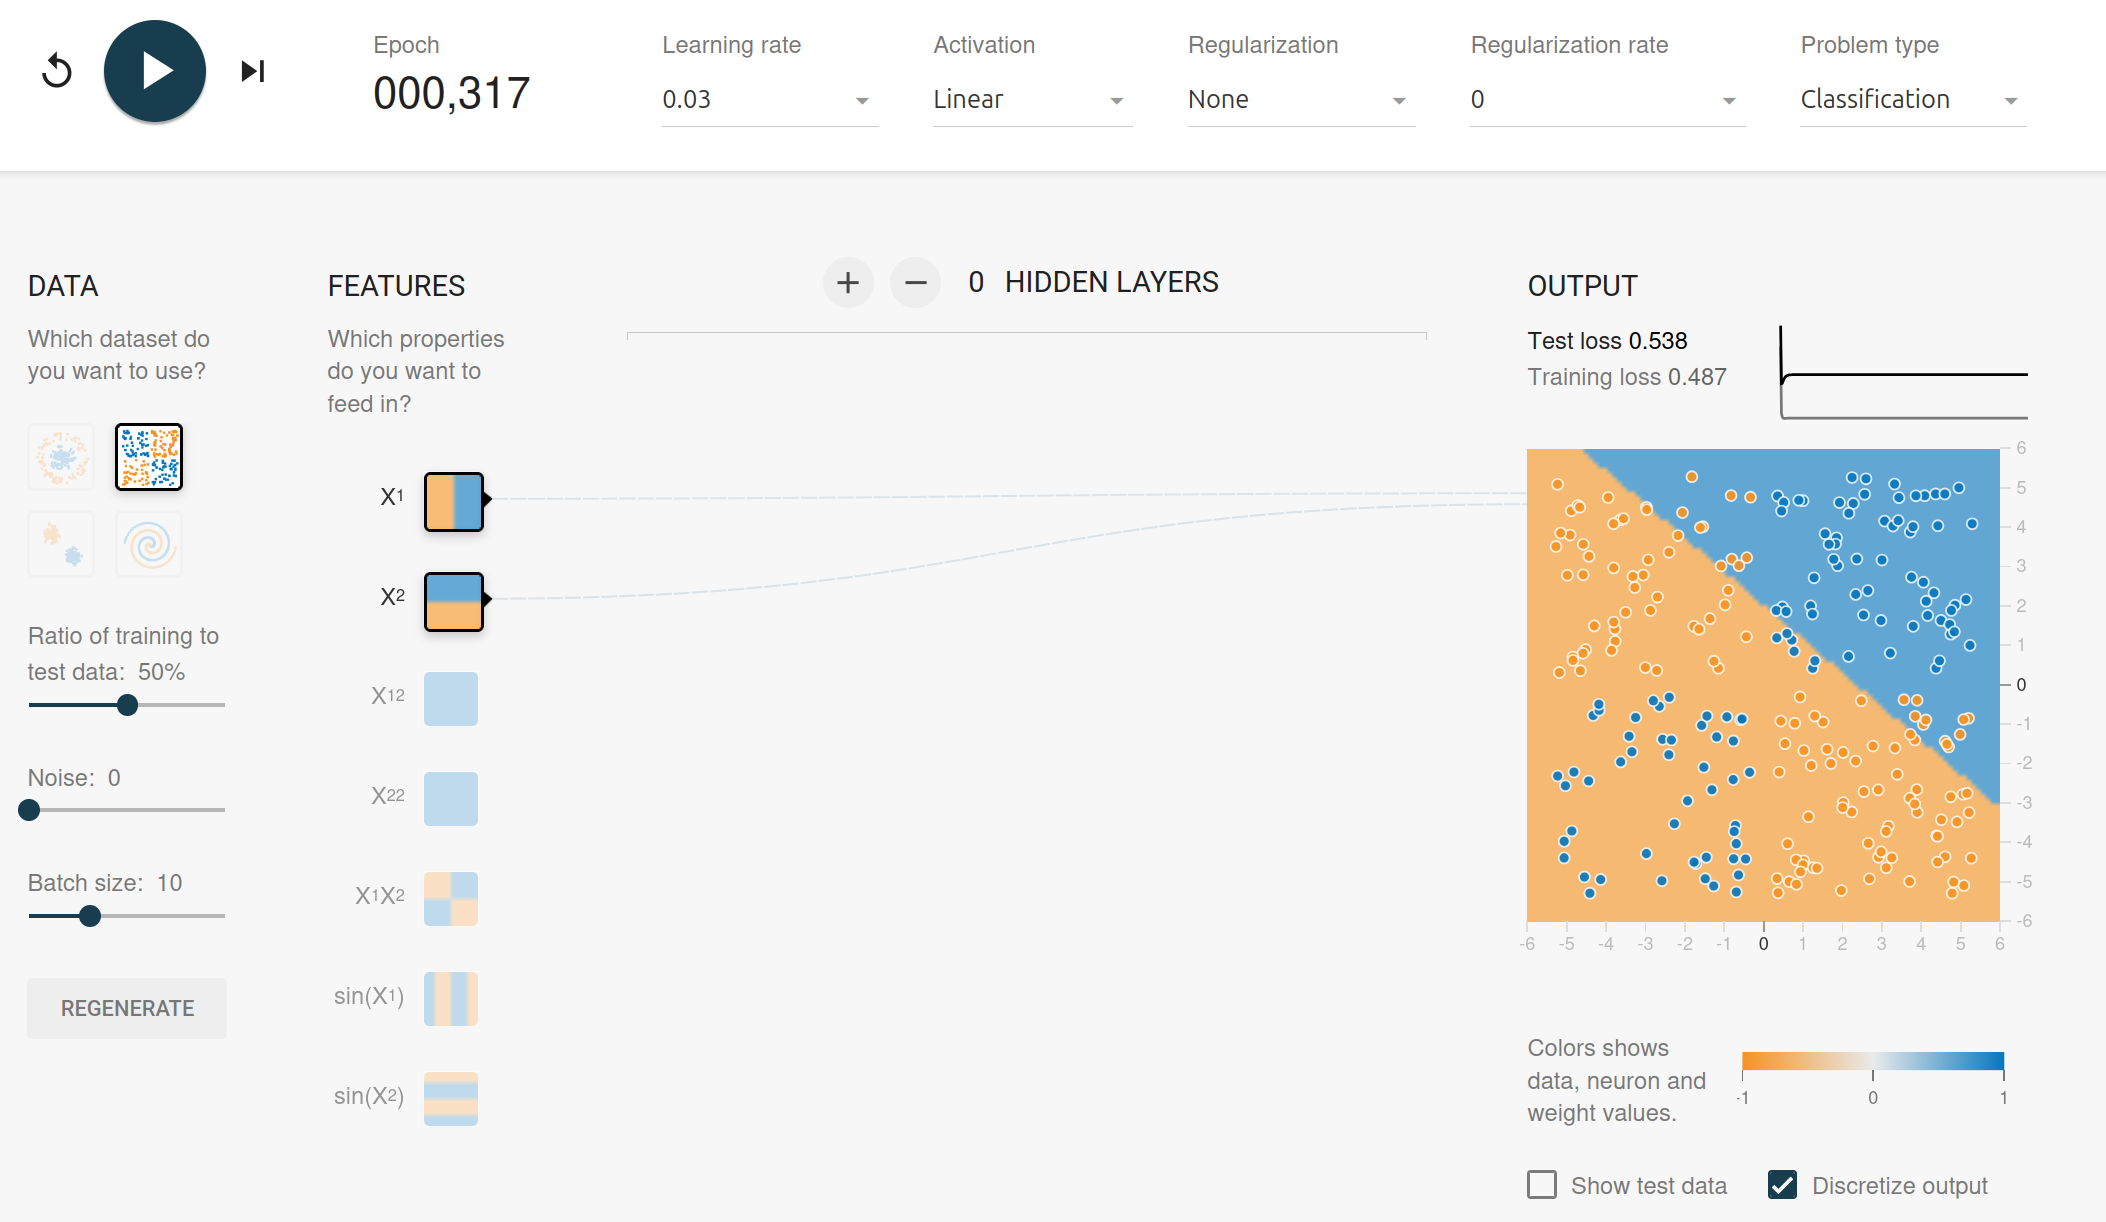
\includegraphics[width = 0.9\linewidth]{img/x1_x2_feat.png}
    \caption{A linear model with no hidden layers using the two independent variables $x_1$ and $x_2$ as features. }
    \label{fig:x1_x2_feat}
\end{figure}
\begin{figure}[htbp]
    \centering
    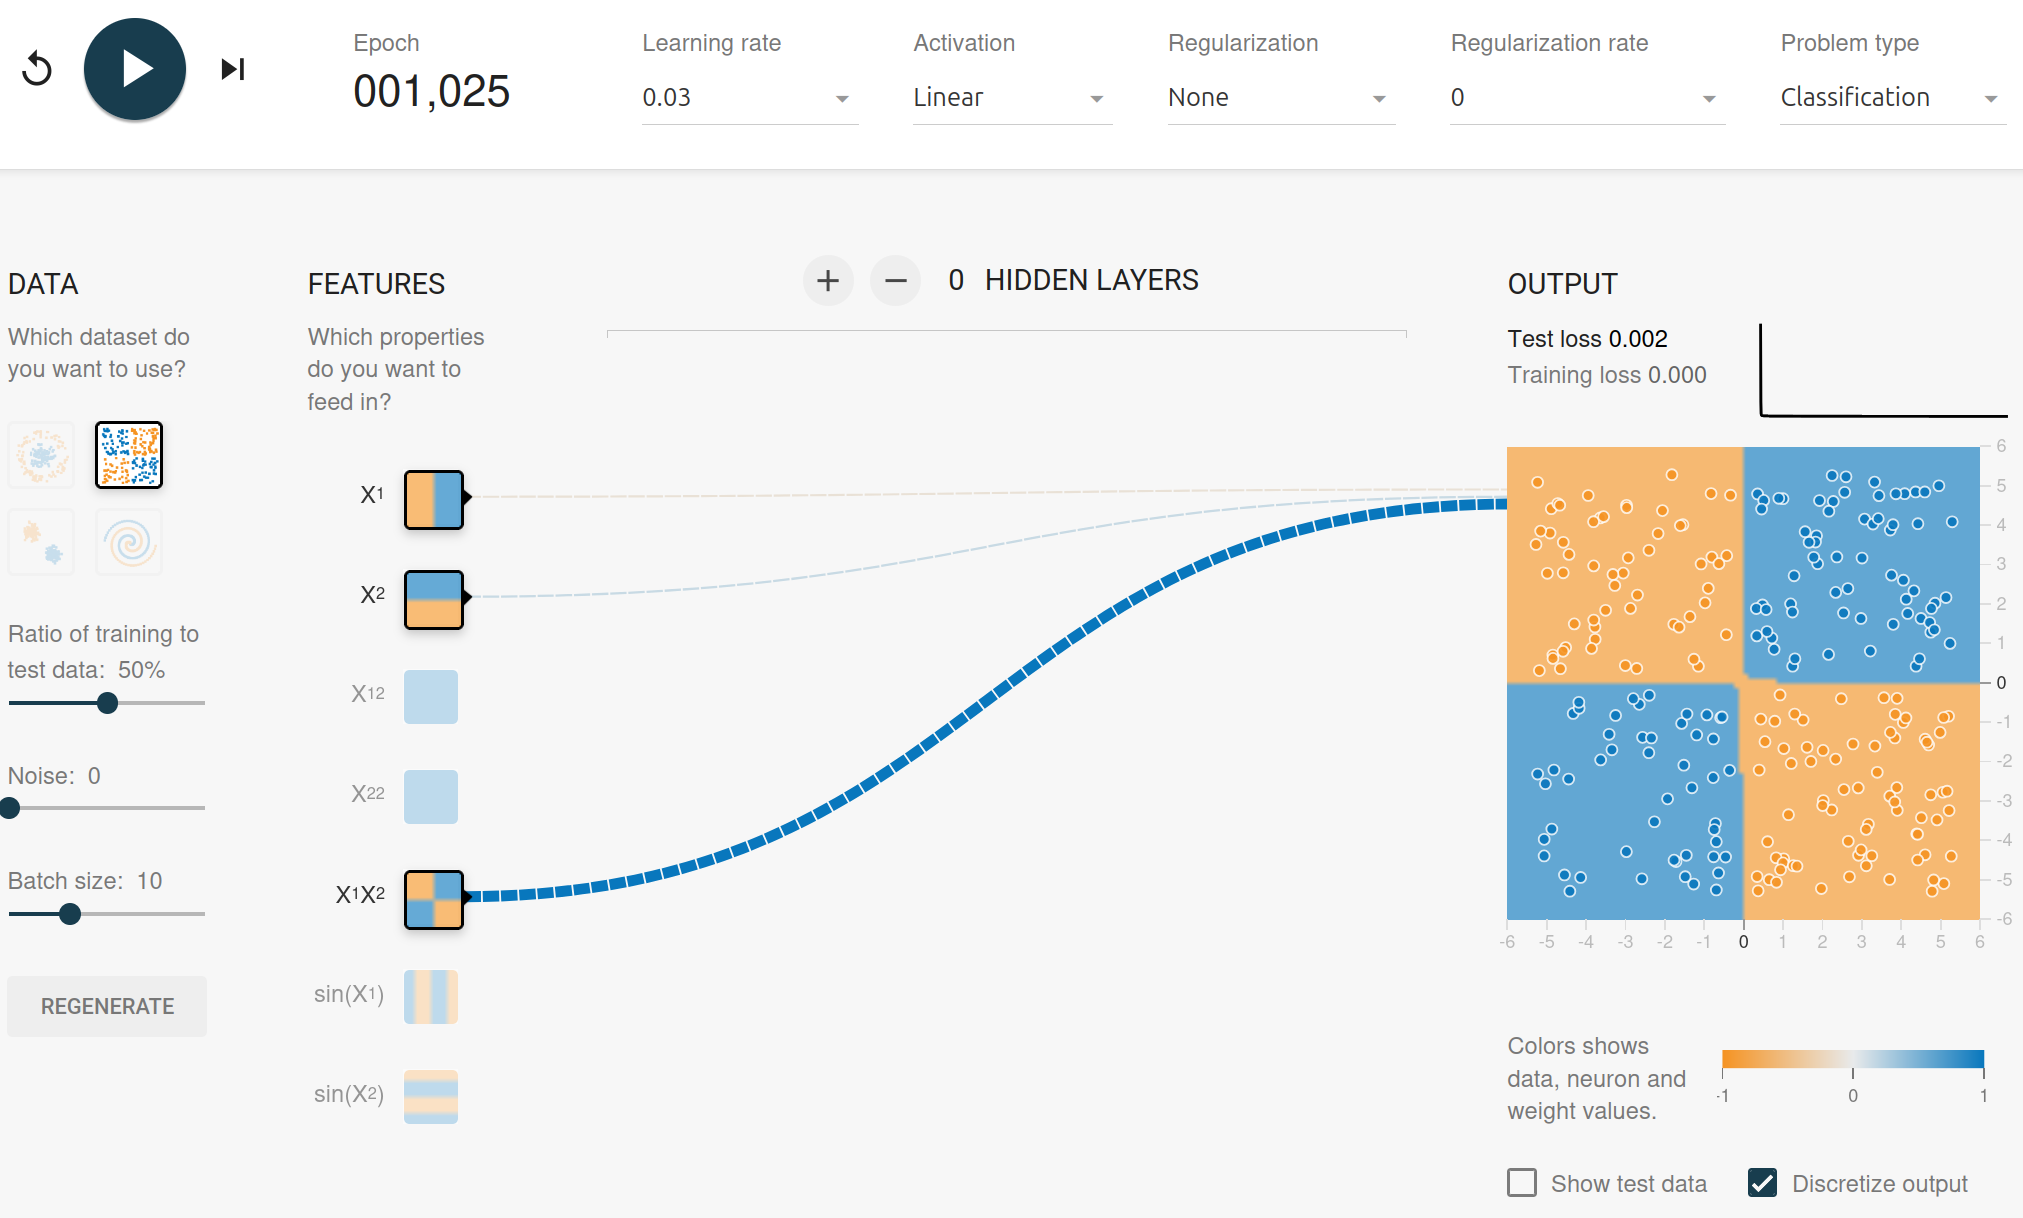
\includegraphics[width = 0.9\linewidth]{img/x1_x2_x1x2_feat.png}
    \caption{A linear model with no hidden layers using $x_1$, $x_2$ and $x_1x_2$ as features. }
    \label{fig:x1_x2_x1x2_feat}
\end{figure}
\newpage

\textit{Now, return the features to just (x1, x2) and start adding hidden layers. What’s the smallest neural network
(least number of layers and least number of neurons per layer) you can create that fits the training data
“perfectly” (i.e. a training loss $<$0.001)? What is the corresponding test loss? Detail your hyperparameter
choices by providing a screenshot and the URL to your solution (the URL contains all your settings choices)}

The smallest neural network that I found able to fit the training data "perfectly" with only $x_1$ and $x_2$ as features used the ReLU activation function. It consisted of a single hidden layer with 4 neurons. The corresponding test loss is 0.002 after  1069 epochs. The result is shown in Figure \ref{fig:x1_x2_perfect}.

\begin{figure}[htbp]
    \centering
    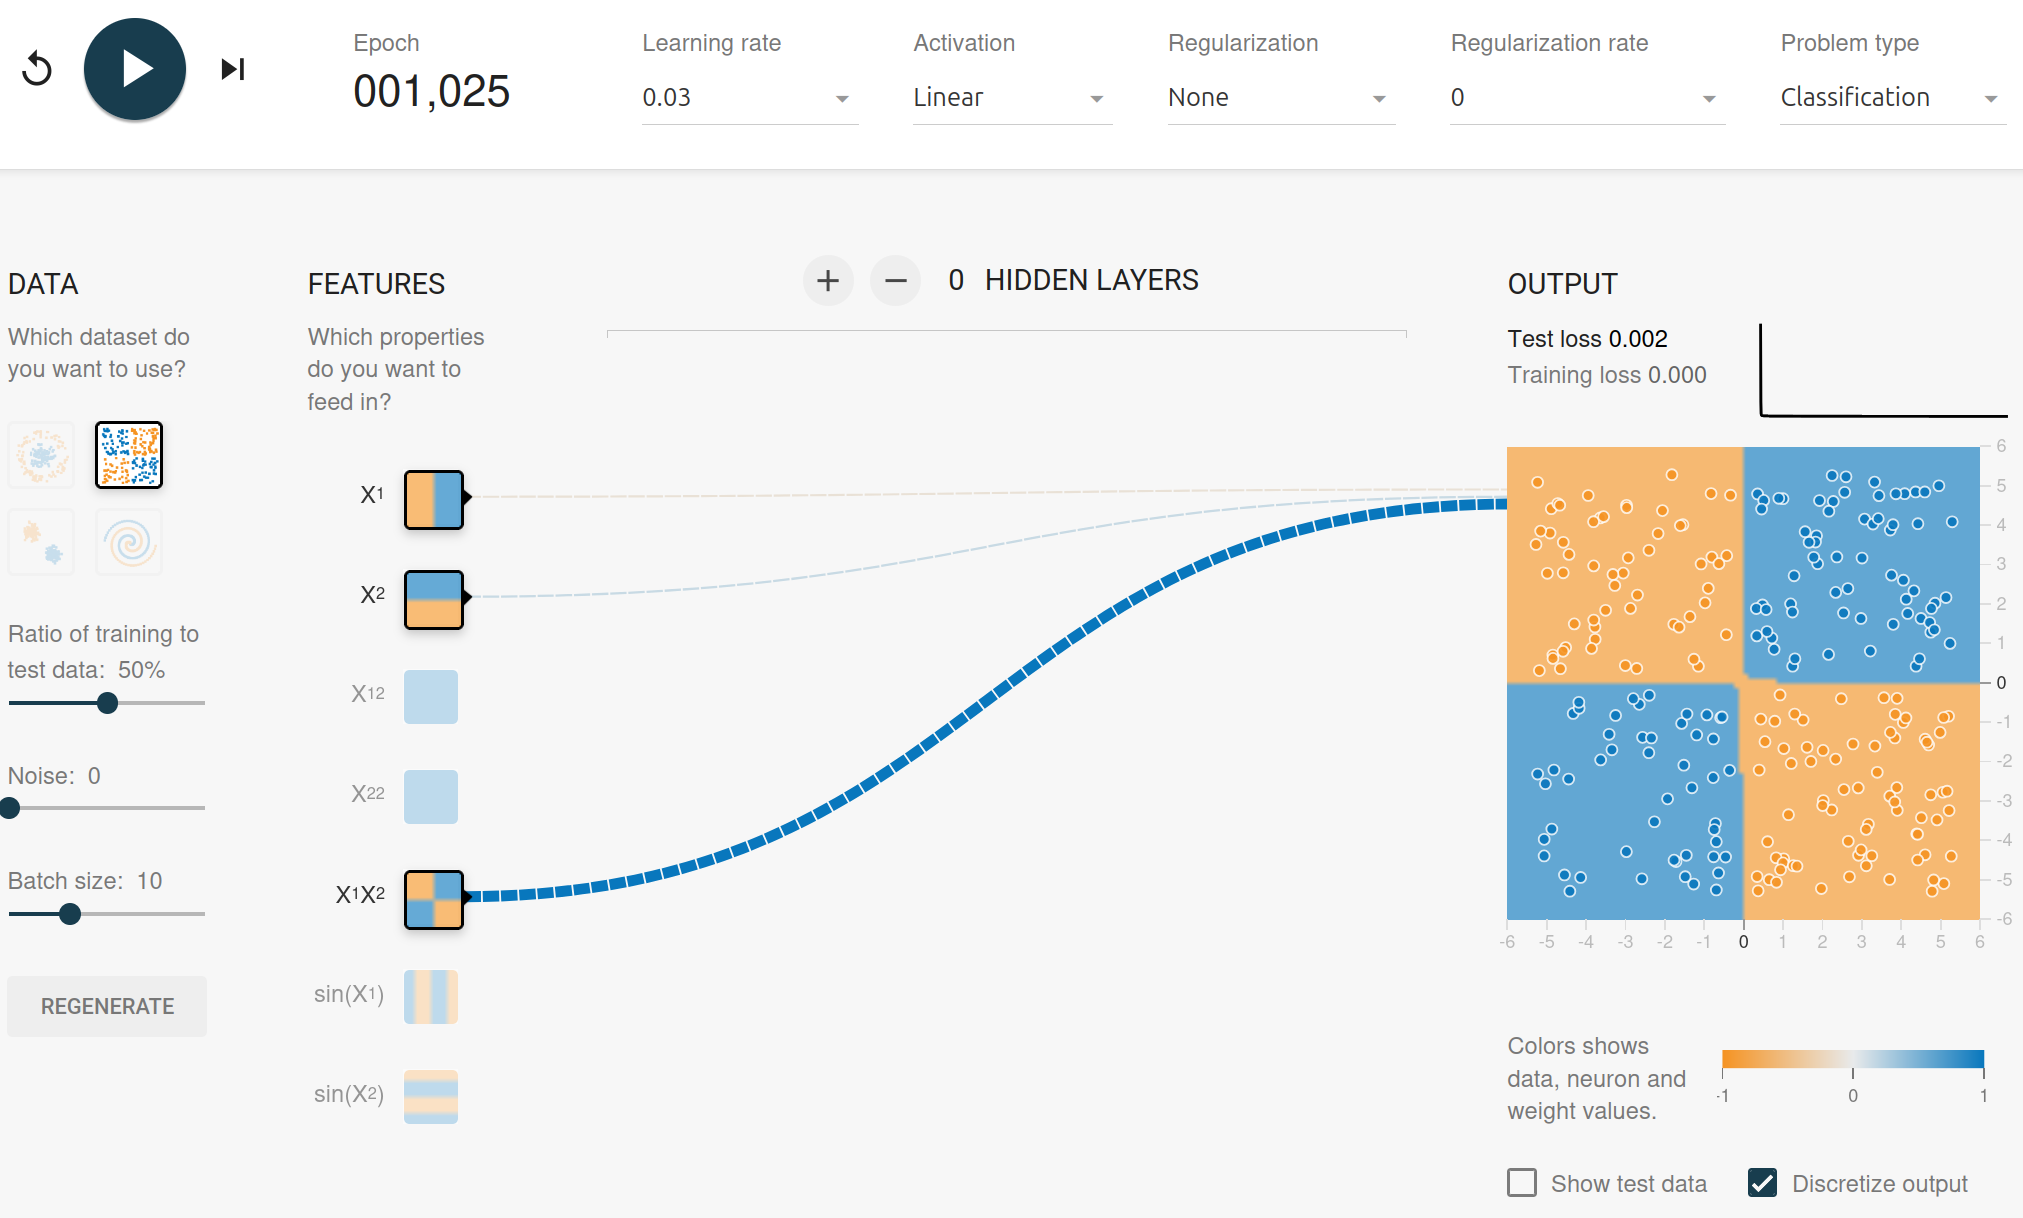
\includegraphics[width = 0.9\linewidth]{img/x1_x2_x1x2_feat.png}
    \caption{The smallest neural network that I found able to fit the training data "perfectly". It uses the ReLU activation funciton and a single hidden layer with 4 neurons. The corresponding test loss is 0.002 after  1069 epochs.}
    \label{fig:x1_x2_perfect}
\end{figure}


















































































